\section{Overview}

This section defines the formal application programming interface (API) and software development kit (SDK) specification for the RCO protocol. The purpose of this specification is to establish a deterministic, verifiable, and reproducible interaction model through which external systems can submit telemetry, verify results, and integrate with the RCO validation pipeline.

Unlike conventional API specifications that focus primarily on request-response formats, the RCO API is defined as a semantic contract. Each API operation is bound to protocol invariants and must preserve deterministic representation, lineage continuity, state consistency, and distributed verification guarantees. As a result, the API is not merely an interface layer but an extension of the protocol itself.

\begin{table}[htbp]
\footnotesize
\centering
\caption{RCO API Endpoint Summary}
\label{tab:api-endpoints}

\renewcommand{\arraystretch}{1.25}

\begin{tabularx}{\textwidth}{|p{3cm}|p{1.8cm}|X|X|p{1.8cm}|X|}
\hline
\textbf{Endpoint} & \textbf{Method} & \textbf{Input Schema} & \textbf{Output Schema} & \textbf{Idempotent} & \textbf{Failure Modes} \\
\hline

\texttt{/v1/ingest} & POST & 
\{\texttt{data}, \texttt{state}, \texttt{metadata}\} &
\{\texttt{status}, \texttt{hash}, \texttt{lineage}, \texttt{proof}\} &
No &
Invalid input, signature failure, insufficient validator quorum \\

\hline

\texttt{/v1/verify} & POST &
\{\texttt{message}, \texttt{proof}\} &
\{\texttt{valid}, \texttt{details}\} &
Yes &
Malformed proof, signature mismatch \\

\hline

\texttt{/v1/lineage/\{id\}} & GET &
Path parameter: \texttt{id} &
\{\texttt{lineage\_chain}\} &
Yes &
Record not found, corrupted lineage \\

\hline

\texttt{/v1/stream} & POST / WS &
\{\texttt{data\_stream}\} &
\{\texttt{status}, \texttt{batch\_proofs}\} &
No &
Stream interruption, batch validation failure \\

\hline

\texttt{/v1/status/\{id\}} & GET &
Path parameter: \texttt{id} &
\{\texttt{status}, \texttt{timestamp}\} &
Yes &
Unknown identifier \\

\hline

\texttt{/v1/health} & GET &
None &
\{\texttt{status}, \texttt{uptime}\} &
Yes &
Service unavailable \\

\hline

\end{tabularx}
\end{table}

The SDK complements this API by abstracting complexity while preserving correctness. It provides developers with structured access to the protocol without requiring direct management of cryptographic primitives, validator coordination, or lineage tracking.

\section{System Boundary Definition}

The API defines the boundary between external systems and the RCO protocol. All interactions must pass through this boundary and conform to its constraints.

Let the external system be denoted as $\mathcal{E}$ and the RCO system as $\mathcal{R}$. The API defines a mapping:

\begin{equation}
\mathcal{A} : \mathcal{E} \rightarrow \mathcal{R}
\end{equation}

such that all inputs $D_t$ from $\mathcal{E}$ are transformed into valid protocol states within $\mathcal{R}$.

No direct mutation of internal state is permitted outside this mapping.

\section{Core Entity Model}

The API operates on a set of well-defined entities. These entities correspond directly to the formal model described in earlier sections.

Telemetry input is defined as $D_t$, representing structured data provided by an external system. This data may include sensor readings, system metrics, or arbitrary structured information.

Canonical representation is defined as $B_t = \mathcal{S}(D_t)$, which is the deterministic encoding of telemetry.

The hash $H_t = \mathcal{H}(B_t)$ uniquely identifies the canonical representation.

Lineage $L_t$ represents the temporal chain linking telemetry events.

System state $S_t$ represents contextual information relevant to telemetry interpretation.

The verification message $M_t$ is constructed from lineage and state.

The proof $\Sigma_t$ represents aggregated validator signatures confirming correctness.

These entities are not independent; they form a tightly coupled structure in which each element depends on the others.

\section{API Interaction Semantics}

Every API call must satisfy the following properties.

First, determinism. Given identical input and state, the API must produce identical outputs. This is critical for reproducibility and verification.

Second, verifiability. Every accepted response must include sufficient information to independently verify correctness without requiring access to internal system state.

Third, immutability. Once a telemetry input is accepted and recorded, it cannot be modified or removed.

Fourth, rejection on uncertainty. If any stage of validation fails or produces ambiguous results, the API must reject the input rather than attempting correction.

\begin{figure}[htbp]
\centering
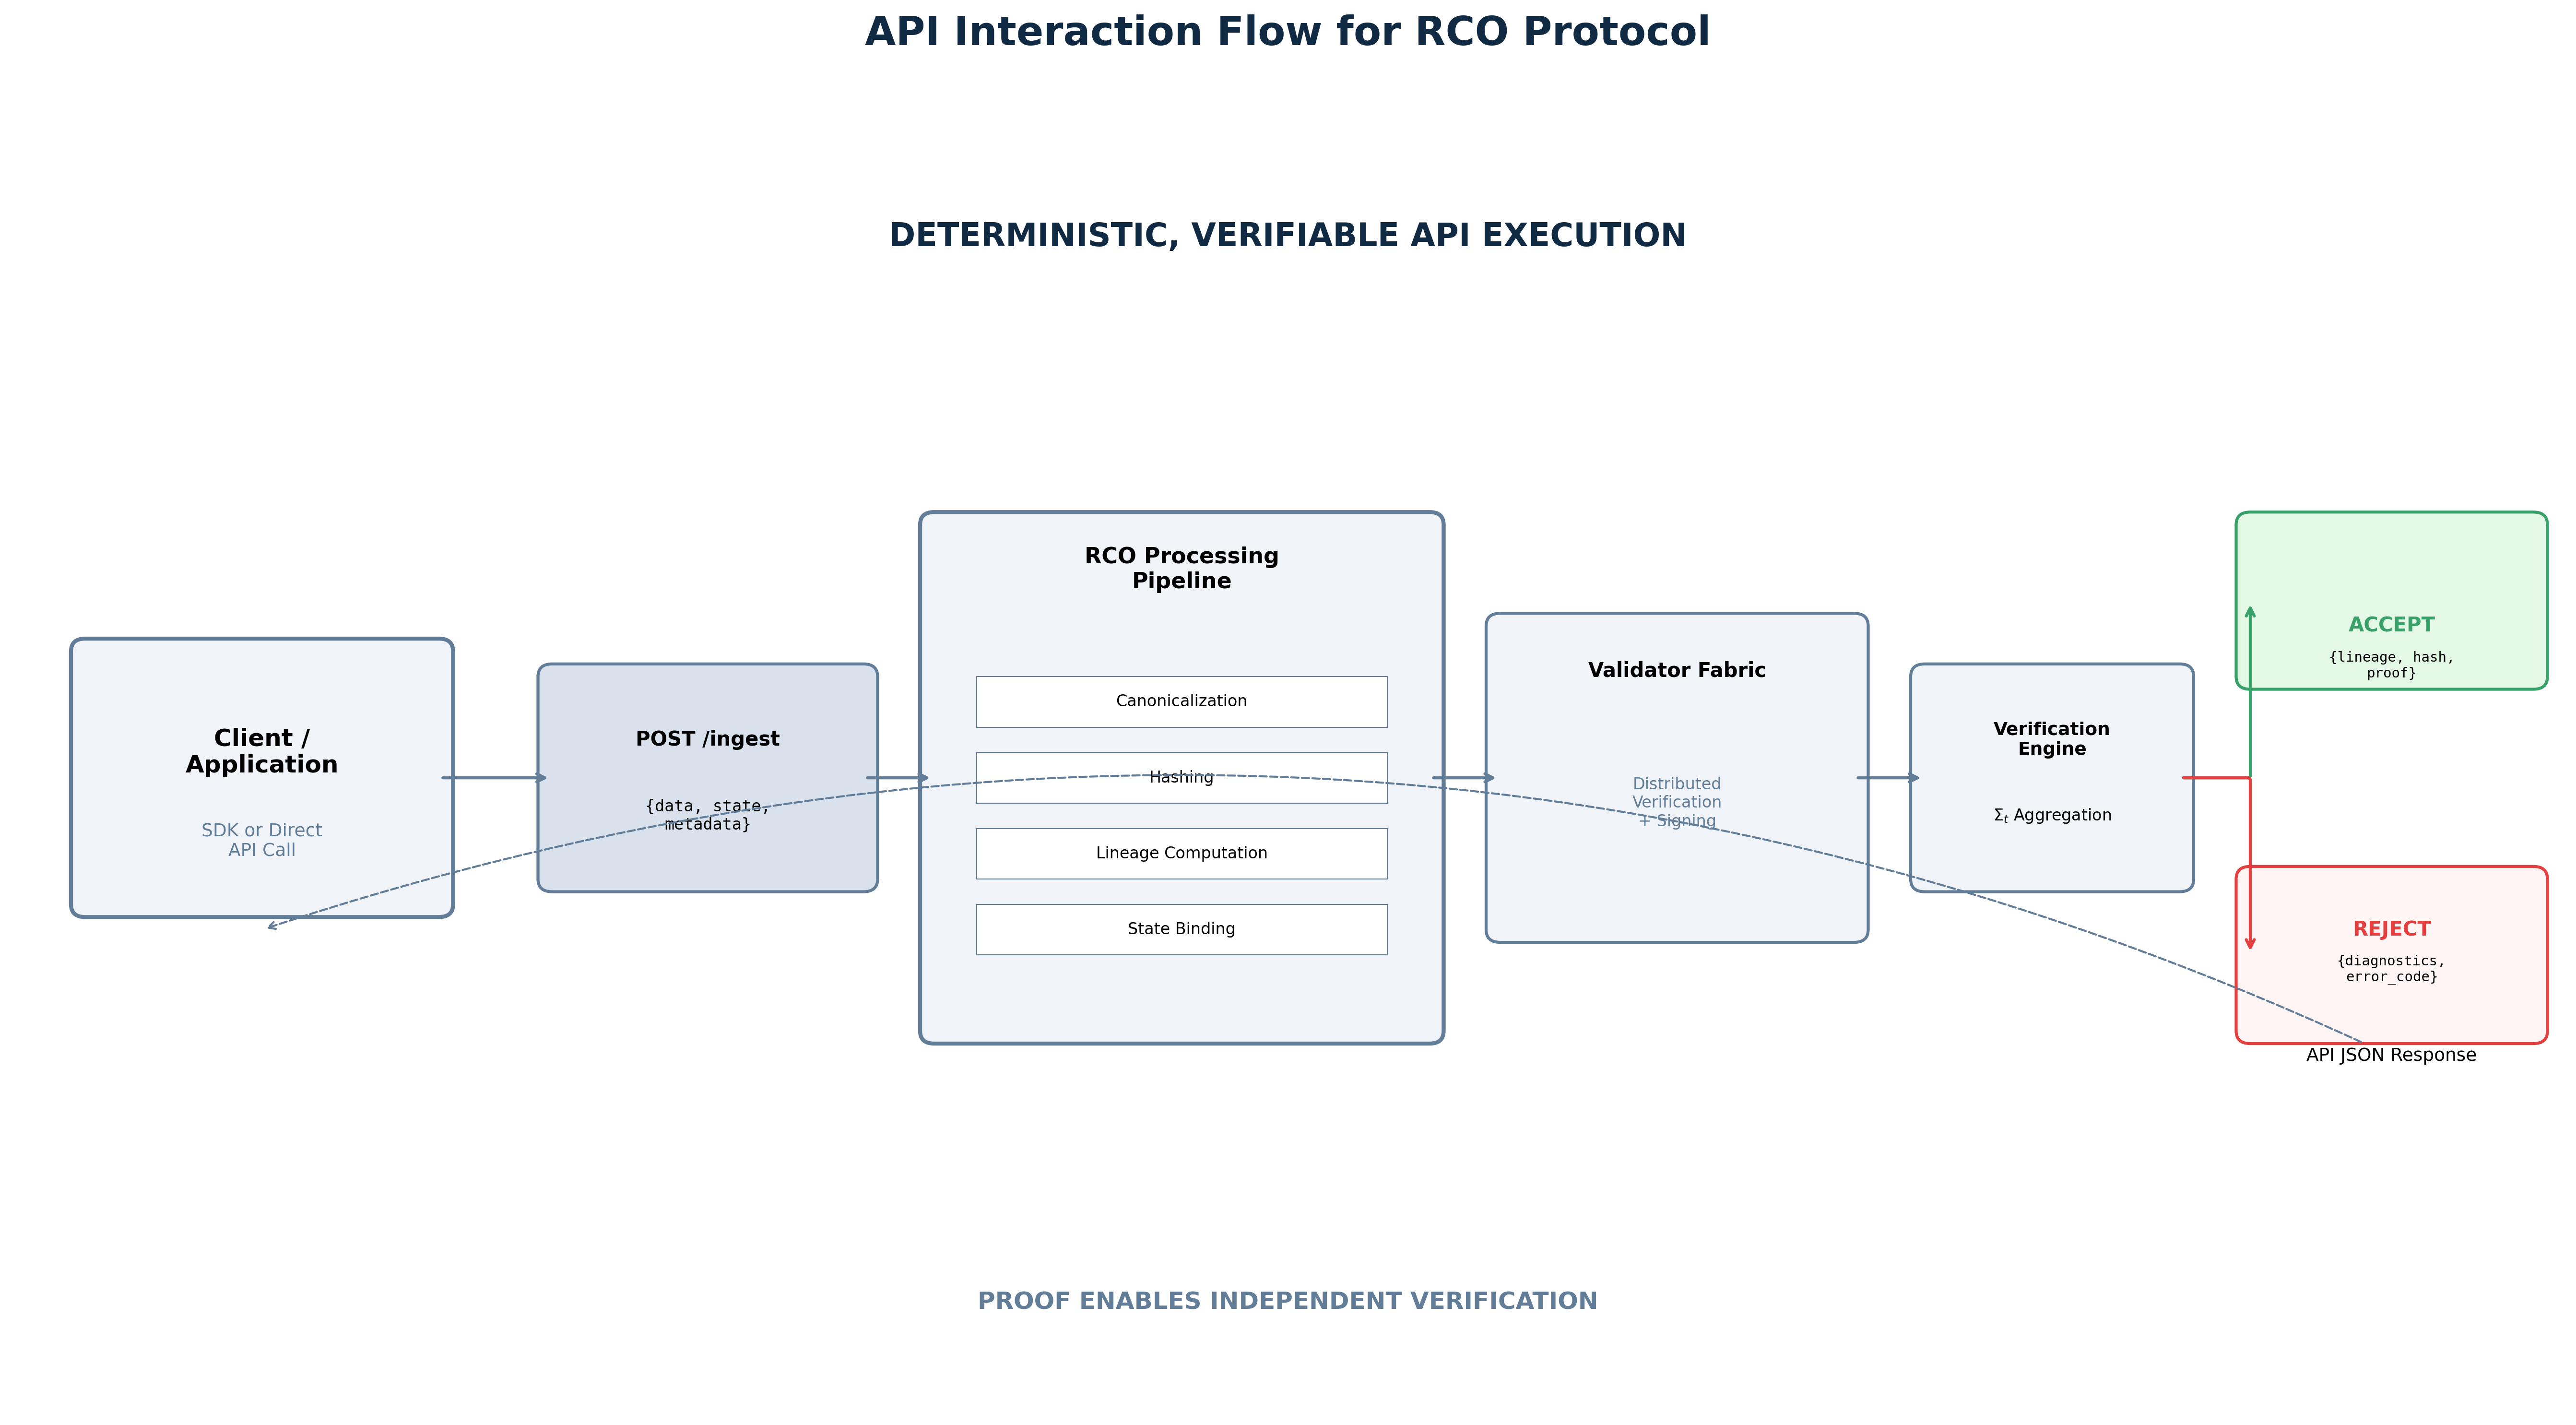
\includegraphics[width=\textwidth]{figures/2-Dimentionals/api_interaction_flow.png}
\caption{API interaction lifecycle from client request through RCO validation pipeline to proof generation and response.}
\label{fig:api}
\end{figure}

\section{Request Lifecycle}

The lifecycle of an API request can be described as a sequence of transformations.

Upon receiving a request, the system first validates the structure of the input. This includes schema validation and type checking.

Next, the input is canonicalized into a deterministic representation. This step eliminates representational ambiguity and ensures consistency across nodes.

The canonical representation is then hashed, producing a fixed-length identifier.

The lineage value is computed by combining the current hash with the previous lineage state.

The system state is hashed and combined with lineage to form the verification message.

This message is distributed to validator nodes, which independently verify and sign it.

The system collects signatures, aggregates them, and verifies the aggregate.

If all conditions are satisfied, the input is accepted and recorded. Otherwise, it is rejected.

\section{State Interaction Model}

The API does not expose direct state mutation operations. Instead, state is implicitly updated through accepted telemetry inputs.

Let the state transition function be:

\begin{equation}
S_{t+1} = \mathcal{F}(S_t, D_t)
\end{equation}

The API enforces that this transition occurs only if $D_t$ is valid.

This ensures that all state transitions are derived from verified inputs, preventing inconsistent or adversarial state evolution.

\section{Idempotency and Replay Behavior}

The API must handle repeated requests in a deterministic manner.

If the same telemetry input is submitted multiple times under identical conditions, the system must produce identical outputs.

However, due to lineage dependency, replaying an input in a different context results in a different lineage value, causing verification to fail.

This ensures that replay attacks are prevented without requiring explicit tracking of request identifiers.

\section{Concurrency Model}

The API supports concurrent requests from multiple clients.

Concurrency is managed through lineage ordering and validator coordination. Each request is processed independently, but lineage ensures that accepted inputs form a consistent sequence.

Conflicts are resolved implicitly through rejection of invalid or inconsistent inputs.

\section{Error Semantics}

Errors are treated as first-class outcomes in the API.

Each error must include:

a clear classification of the error type;

the stage at which the error occurred;

sufficient information to diagnose the issue.

Errors are not hidden or automatically corrected. This design choice ensures transparency and prevents silent failures.

\section{Security Model}

All API interactions must be authenticated and encrypted. The API assumes a secure transport layer and may include additional authentication mechanisms such as API keys or token-based access.

Authorization policies may restrict access to specific endpoints or operations.

The API must also enforce rate limiting and input validation to prevent abuse.

\section{Extensibility}

The API is designed to be extensible. New fields, endpoints, and features may be added without breaking existing functionality.

This is achieved through versioning and backward-compatible schema evolution.

\section{Conclusion}

This section establishes the foundational model for the RCO API and SDK. By defining entities, semantics, and interaction constraints in detail, it ensures that all external interactions with the system are consistent, verifiable, and aligned with protocol guarantees. This foundation supports the development of more specific endpoint definitions and SDK abstractions in subsequent sections.

\section{General API Conventions}

All API endpoints follow a consistent structure and set of conventions to ensure interoperability and predictability.

All requests and responses are encoded using JSON with UTF-8 encoding. Field names are case-sensitive and follow a standardized naming convention using lowercase with underscores.

All timestamps are represented in ISO 8601 format. All identifiers are treated as opaque strings and must not be interpreted by clients unless explicitly specified.

Each request must include a metadata block that provides contextual information about the request. This metadata is used for auditing, traceability, and validation.

\section{Ingestion Endpoint Specification}

\subsection{Endpoint Definition}

\begin{verbatim}
POST /v1/ingest
\end{verbatim}

\subsection{Request Schema}

\begin{verbatim}
{
  "data": {
    "type": "object",
    "required": true,
    "description": "Telemetry payload"
  },
  "state": {
    "type": "object",
    "required": true,
    "description": "System state context"
  },
  "metadata": {
    "timestamp": "string (ISO 8601)",
    "source_id": "string",
    "schema_version": "string",
    "request_id": "string"
  }
}
\end{verbatim}

\subsection{Field Semantics}

The \texttt{data} field contains the telemetry input. It must be a structured object with deterministic key-value pairs.

The \texttt{state} field represents the contextual system state. This must reflect the current state from which the telemetry was generated.

The \texttt{metadata} field provides additional context. The \texttt{request\_id} must be unique per request to support traceability.

\subsection{Validation Rules}

The ingestion endpoint enforces strict validation rules.

The \texttt{data} object must not contain non-deterministic structures such as unordered collections or floating-point values without normalization.

The \texttt{state} object must be consistent with the system’s expected state schema.

The \texttt{metadata.timestamp} must be within an acceptable time window to prevent stale or future-dated inputs.

Duplicate \texttt{request\_id} values may be rejected or treated as idempotent operations depending on configuration.

\subsection{Processing Semantics}

Upon receiving a valid request, the system performs canonicalization, hashing, lineage computation, state binding, and distributed verification.

If any stage fails, the request is rejected.

\subsection{Response Schema}

\begin{verbatim}
{
  "status": "accept" | "reject",
  "result": {
    "lineage": "string",
    "hash": "string",
    "message": "string",
    "proof": {
      "type": "threshold_signature",
      "validator_count": "integer",
      "signatures": [
        {
          "validator_id": "string",
          "signature": "string"
        }
      ]
    }
  },
  "diagnostics": {
    "stage": "string",
    "error_code": "string",
    "message": "string"
  }
}
\end{verbatim}

\subsection{Response Semantics}

If the status is \texttt{accept}, the result block contains all necessary information for verification.

If the status is \texttt{reject}, the diagnostics block provides detailed information about the failure.

\section{Verification Endpoint Specification}

\subsection{Endpoint Definition}

\begin{verbatim}
POST /v1/verify
\end{verbatim}

\subsection{Request Schema}

\begin{verbatim}
{
  "message": "string",
  "proof": {
    "type": "threshold_signature",
    "signatures": [...]
  },
  "public_keys": [
    {
      "validator_id": "string",
      "key": "string"
    }
  ]
}
\end{verbatim}

\subsection{Validation Rules}

The message must be well-formed and correspond to a valid state-lineage binding.

The number of provided signatures must meet or exceed the threshold requirement.

Each signature must correspond to a valid public key.

\subsection{Response Schema}

\begin{verbatim}
{
  "valid": true | false,
  "details": {
    "verified_signatures": "integer",
    "required_threshold": "integer"
  }
}
\end{verbatim}

\subsection{Behavior}

The endpoint verifies each signature independently and ensures that the threshold condition is satisfied.

\section{Lineage Query Endpoint}

\subsection{Endpoint Definition}

\begin{verbatim}
GET /v1/lineage/{lineage_id}
\end{verbatim}

\subsection{Response Schema}

\begin{verbatim}
{
  "lineage": "string",
  "previous": "string",
  "timestamp": "string",
  "hash": "string",
  "state_hash": "string"
}
\end{verbatim}

\subsection{Behavior}

This endpoint returns lineage information for auditing and traceability.

\section{Streaming Endpoint}

\subsection{Endpoint Definition}

\begin{verbatim}
POST /v1/stream
\end{verbatim}

\subsection{Request Schema}

\begin{verbatim}
{
  "stream_id": "string",
  "events": [
    {
      "data": { ... },
      "state": { ... },
      "metadata": { ... }
    }
  ]
}
\end{verbatim}

\subsection{Processing Semantics}

Each event in the stream is processed sequentially, maintaining lineage continuity.

Failures in any event may result in rejection of that event or the entire batch depending on configuration.

\section{Error Codes}

The API defines standardized error codes.

\begin{verbatim}
VALIDATION_ERROR
CANONICALIZATION_ERROR
HASH_MISMATCH
LINEAGE_ERROR
SIGNATURE_INSUFFICIENT
SIGNATURE_INVALID
TIMEOUT
INTERNAL_ERROR
\end{verbatim}

Each error code corresponds to a specific stage in the pipeline.

\section{Edge Case Handling}

The API explicitly defines behavior for edge cases.

Empty data payloads are rejected unless explicitly allowed by schema.

Large payloads exceeding size limits are rejected.

Partial validator responses result in rejection if the threshold is not met.

Network timeouts trigger retry logic but do not compromise correctness.

\begin{table}[htbp]
\footnotesize
\centering
\caption{RCO API Error Codes and Failure Semantics}
\label{tab:error-codes}

\renewcommand{\arraystretch}{1.25}

\begin{tabularx}{\textwidth}{|p{2cm}|p{3cm}|X|X|X|}
\hline
\textbf{Code} & \textbf{Error Name} & \textbf{Description} & \textbf{System Action} & \textbf{Client Action} \\
\hline

400 & Invalid Input & Malformed or schema-invalid request payload & Request rejected before processing & Fix request format and retry \\

\hline

401 & Unauthorized & Missing or invalid authentication credentials & Request blocked at API gateway & Provide valid credentials \\

\hline

403 & Forbidden & Authenticated but not permitted for operation & Request denied & Check permissions \\

\hline

404 & Not Found & Requested resource or lineage ID does not exist & No processing performed & Verify identifier \\

\hline

409 & Conflict & Duplicate or conflicting ingestion request & Request rejected to maintain consistency & Avoid duplicate submissions \\

\hline

422 & Validation Failed & RCO validation failed (hash mismatch, state inconsistency, lineage error) & Telemetry rejected (not persisted) & Inspect diagnostics and correct data \\

\hline

429 & Rate Limited & Too many requests or ingestion overload & Request throttled & Retry with backoff \\

\hline

500 & Internal Error & Unexpected failure in processing pipeline & Processing aborted & Retry or contact support \\

\hline

502 & Validator Failure & Insufficient valid signatures or validator errors & Validation aborted & Retry after delay \\

\hline

503 & Service Unavailable & System temporarily unavailable (maintenance or overload) & Request not processed & Retry later \\

\hline

504 & Timeout & Validation or aggregation exceeded time limits & Request terminated & Retry with adjusted parameters \\

\hline

\end{tabularx}
\end{table}

\section{Schema Evolution}

The API supports schema evolution through versioning.

New fields may be added as optional fields.

Existing fields must not change semantics.

Deprecated fields must be supported for a defined transition period.

\section{Conclusion}

This section defines the detailed endpoint specifications, schemas, and validation rules for the RCO API. By providing explicit definitions and handling edge cases, the specification ensures that the API can be implemented consistently across different environments while preserving the protocol’s guarantees.

\section{SDK Design, Client Lifecycle, and Integration Patterns}

\section{Overview}

This section defines the structure, behavior, and lifecycle of the SDK used to interact with the RCO API. While the API provides a protocol-level interface, the SDK encapsulates complexity and enforces correct usage patterns at the client level.

The SDK is designed to operate across multiple programming languages and runtime environments. It provides a consistent abstraction over canonicalization, hashing, lineage tracking, request orchestration, and response verification. The SDK must preserve all protocol invariants while optimizing for performance, usability, and fault tolerance.

\section{SDK Design Principles}

The SDK is governed by several core design principles.

First, correctness by construction. The SDK must prevent invalid API usage by enforcing schema validation, deterministic processing, and protocol sequencing internally.

Second, minimal trust assumptions. The SDK must not rely on external systems for correctness and must independently verify all responses received from the API.

Third, transparency of operations. All internal transformations, including canonicalization and hashing, must be reproducible and optionally inspectable for debugging and auditing.

Fourth, adaptability. The SDK must support multiple deployment environments, including synchronous and asynchronous execution models, as well as resource-constrained environments.

\section{Core SDK Abstraction}

The SDK exposes a primary client abstraction that encapsulates interaction with the RCO system.

\begin{verbatim}
class RCOClient:
    def __init__(self, config):
        self.endpoint = config.endpoint
        self.keys = config.keys
        self.lineage = config.initial_lineage
        self.cache = {}
\end{verbatim}

The client maintains internal state, including lineage and optional caches, while exposing high-level operations such as ingestion and verification.

\section{Client Lifecycle}

The lifecycle of the SDK client follows a well-defined sequence.

Upon initialization, the client loads configuration parameters, including endpoint URLs, cryptographic keys, and initial lineage state.

During operation, the client processes telemetry inputs through a local pipeline that may include canonicalization and hashing before submitting requests to the API.

After receiving a response, the client verifies the returned proof and updates its internal lineage state if the operation is accepted.

The lifecycle ensures that the client remains synchronized with the system while preserving determinism.

\section{Local Preprocessing}

The SDK may perform preprocessing steps locally to reduce network overhead and improve performance.

These steps include deterministic canonicalization of input data and optional pre-hashing.

\begin{verbatim}
def preprocess(data):
    serialized = canonicalize(data)
    return hash_data(serialized)
\end{verbatim}

Local preprocessing must produce results identical to server-side processing to maintain consistency.

\section{Retry and Failure Handling}

The SDK includes built-in mechanisms for handling transient failures.

If a request fails due to network issues or timeouts, the SDK may retry the request with exponential backoff.

\begin{verbatim}
def retry_request(fn, retries=3):
    for i in range(retries):
        try:
            return fn()
        except Exception:
            sleep(2 ** i)
    raise Exception("Request failed")
\end{verbatim}

Retries must not violate idempotency or introduce inconsistencies.

\section{Batch Processing}

The SDK supports batching of multiple telemetry inputs to improve throughput.

\begin{verbatim}
def batch_ingest(events):
    results = []
    for event in events:
        results.append(self.ingest(event.data, event.state))
    return results
\end{verbatim}

Batch processing must preserve ordering when required and maintain lineage continuity across events.

\section{Client-Side Lineage Management}

The SDK maintains a local copy of lineage state to ensure consistency across requests.

After each accepted operation, the lineage is updated.

\begin{verbatim}
if result["status"] == "accept":
    self.lineage = result["lineage"]
\end{verbatim}

This local state must remain consistent with the server. In case of divergence, the SDK must resynchronize using lineage query endpoints.

\section{Caching Strategies}

The SDK may cache intermediate results to improve performance.

Examples include caching canonical representations, hashes, and recent lineage states.

Caching must not compromise correctness. Cached values must be invalidated if underlying data changes.

\section{Asynchronous SDK Design}

For high-throughput systems, the SDK provides asynchronous interfaces.

\begin{verbatim}
async def ingest_async(data, state):
    return await api_call(data, state)
\end{verbatim}

Asynchronous execution allows concurrent processing of multiple requests without blocking.

\section{Multi-Language Support}

The SDK is designed to be implemented across multiple programming languages.

Each implementation must adhere to the same canonicalization rules, hashing algorithms, and request formats.

Language-specific differences must not affect protocol behavior.

\section{Integration Patterns}

The SDK supports multiple integration patterns.

In a microservices architecture, the SDK may be embedded within each service that produces telemetry. This allows direct interaction with the RCO API.

In an event-driven architecture, the SDK may process events from message queues and submit them for validation.

\begin{figure}[htbp]
\centering
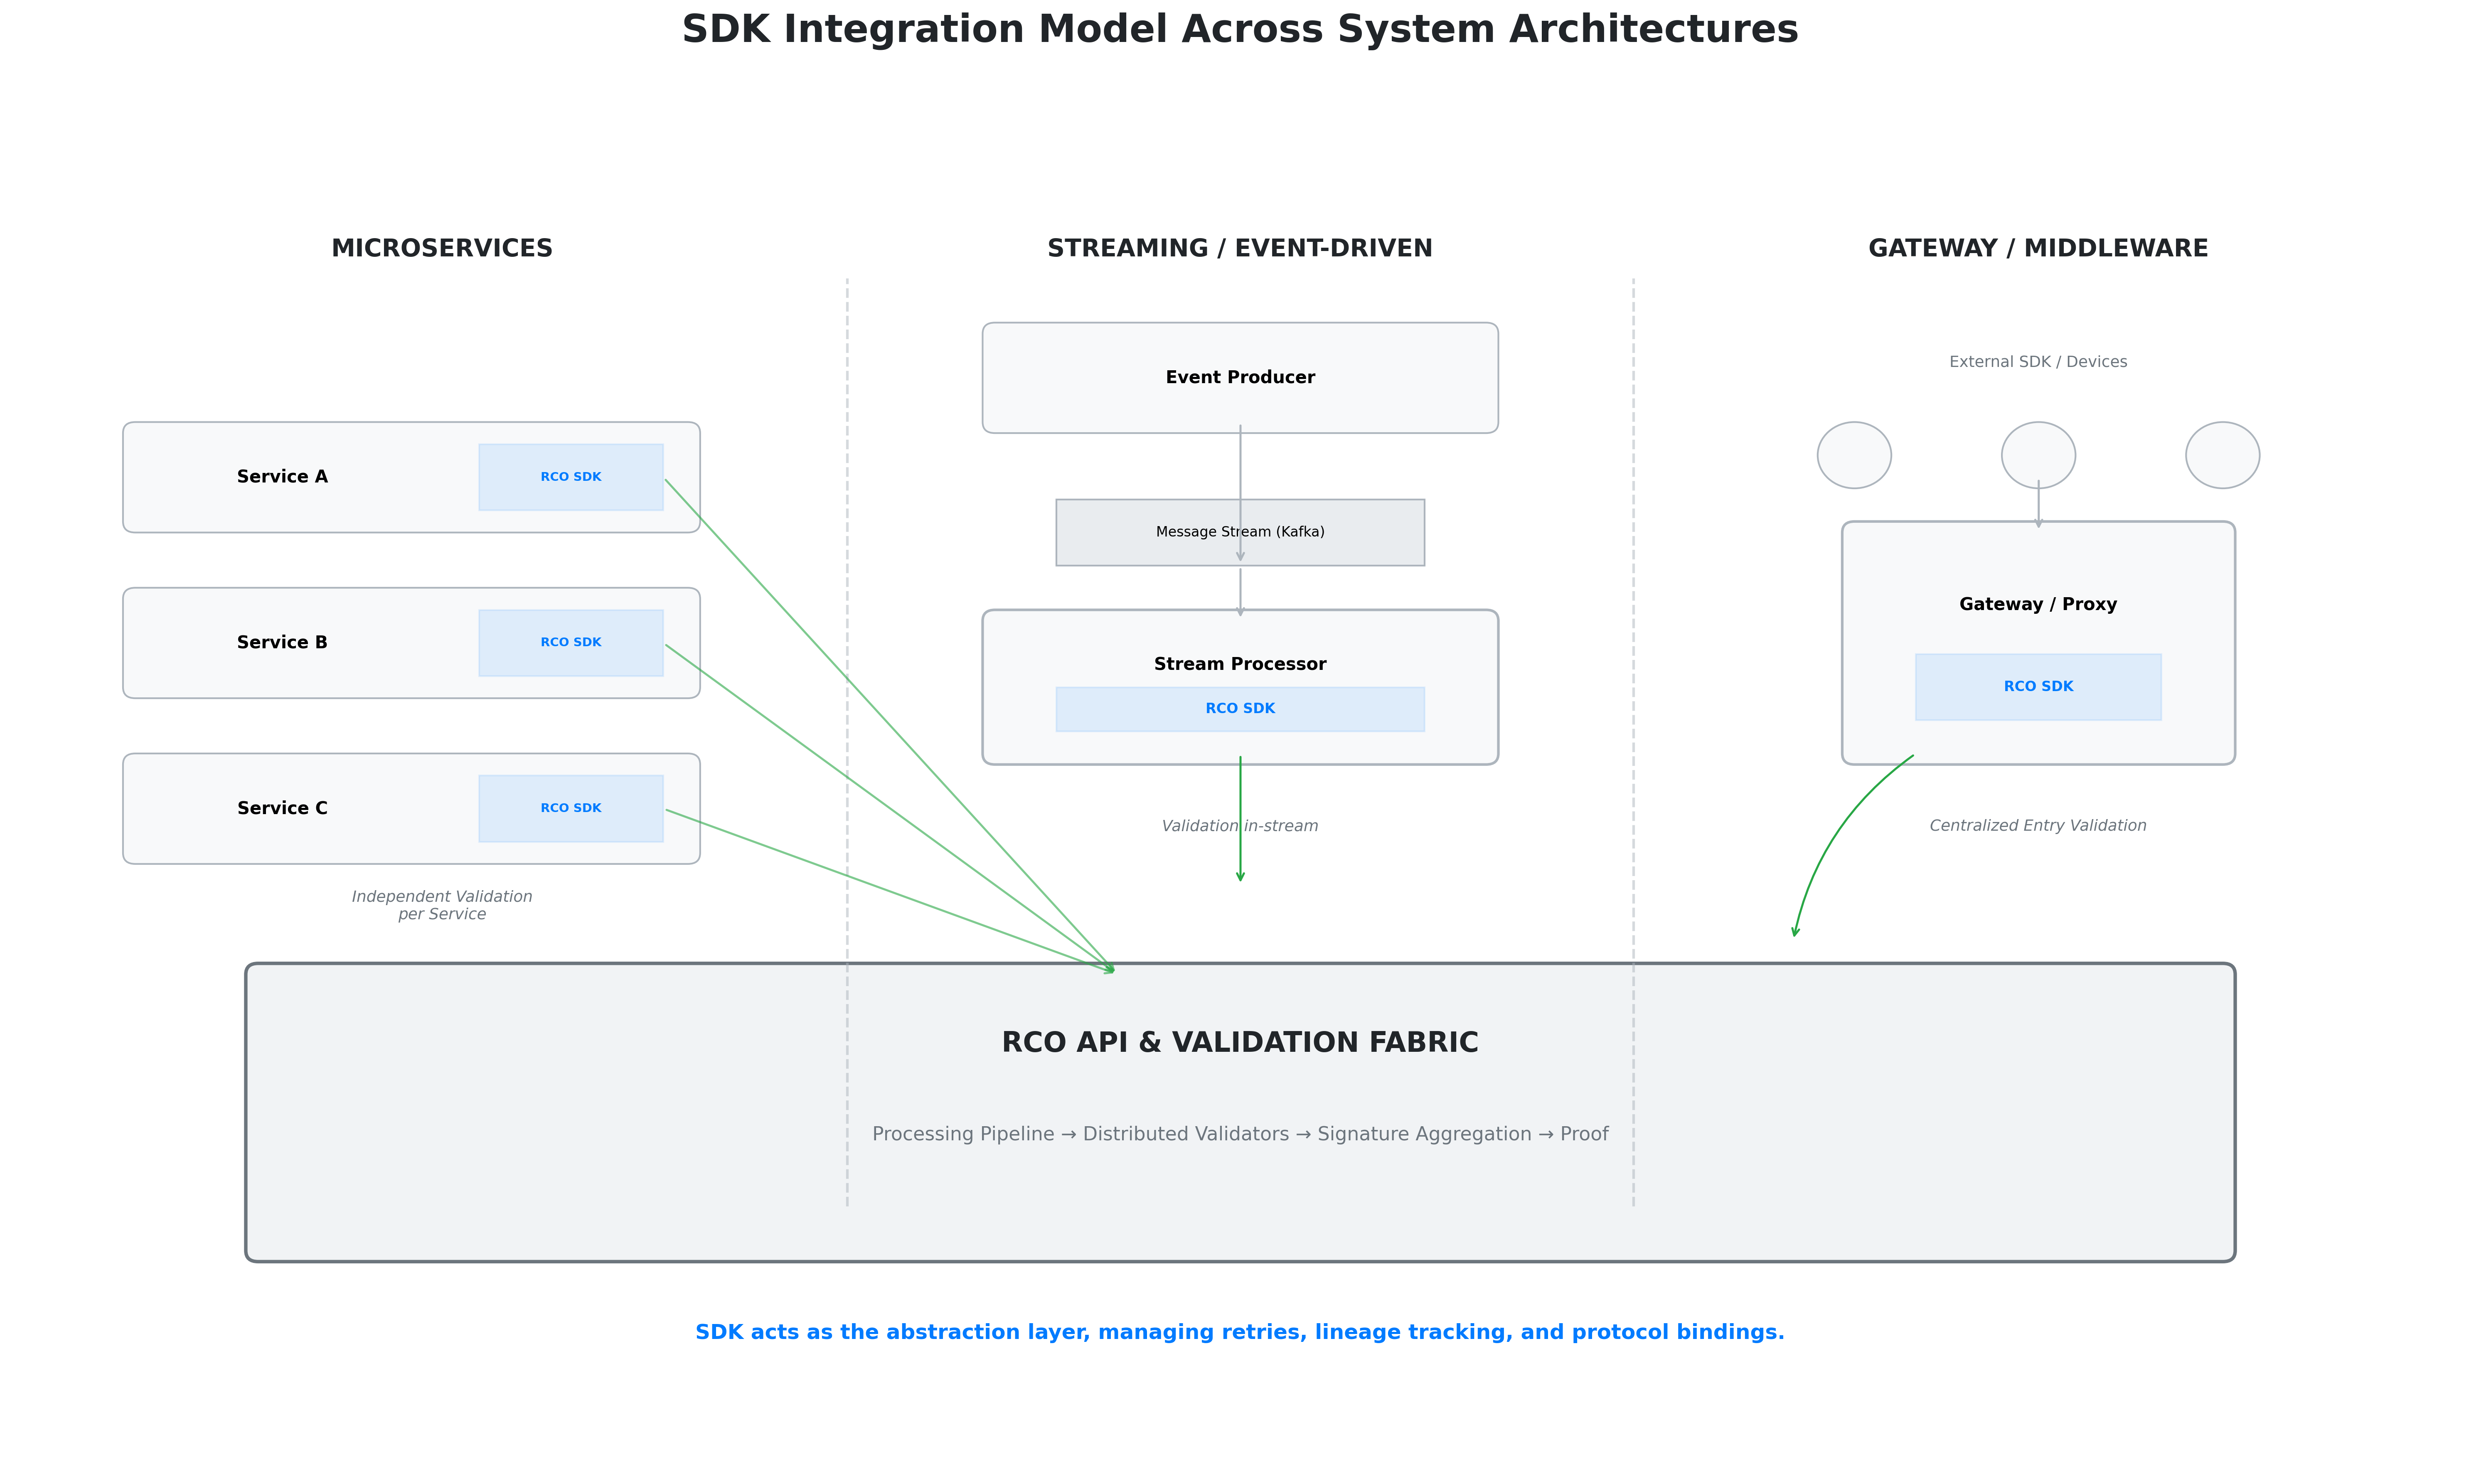
\includegraphics[width=\textwidth]{figures/2-Dimentionals/sdk_integration_model.png}
\caption{SDK integration across microservices, streaming systems, and middleware architectures enabling seamless adoption of RCO.}
\label{fig:sdk}
\end{figure}

In a centralized architecture, a dedicated service may act as a gateway, using the SDK to process all incoming telemetry.

\section{Middleware Integration}

The SDK can function as middleware between data producers and consumers.

In this role, it intercepts telemetry, validates it using the RCO protocol, and forwards only accepted data downstream.

\section{Streaming Integration}

For streaming systems, the SDK processes continuous data flows.

It maintains lineage across events and ensures that each event is validated in sequence.

\section{Backpressure and Flow Control}

The SDK must handle backpressure in high-load scenarios.

If the API cannot process requests fast enough, the SDK may queue requests or throttle input rates.

This prevents system overload and maintains stability.

\section{Security Considerations}

The SDK must securely manage cryptographic keys and ensure that sensitive data is not exposed.

All communication with the API must be encrypted.

The SDK must also validate all responses to prevent tampering.

\section{Observability}

The SDK provides hooks for logging and monitoring.

\begin{verbatim}
def log(event):
    print("[RCO SDK]", event)
\end{verbatim}

These hooks allow integration with external monitoring systems.

\section{Conclusion}

This section defines the SDK design and integration patterns for the RCO protocol. By providing a structured and robust client abstraction, the SDK enables developers to integrate the protocol into a wide range of systems while preserving correctness and performance. The combination of lifecycle management, caching, asynchronous execution, and integration flexibility ensures that the SDK is suitable for production environments.

\section{Authentication, Authorization, Observability, and Governance}

\section{Overview}

This section defines the control plane of the RCO API. While previous sections established functional correctness and interaction semantics, this section addresses operational security, access control, observability, and compliance requirements. These elements are essential for deploying the protocol in production environments where accountability, traceability, and controlled access are mandatory.

The design ensures that all interactions with the system are authenticated, authorized, rate-limited, observable, and auditable without compromising the protocol’s core guarantees.

\section{Authentication Model}

All API requests must be authenticated. The system supports multiple authentication mechanisms to accommodate different deployment environments.

Authentication is performed at the API gateway layer and must precede any processing of telemetry inputs.

Supported authentication mechanisms include token-based authentication, API keys, and cryptographic identity-based authentication.

\subsection{Token-Based Authentication}

Clients may authenticate using bearer tokens.

\begin{verbatim}
Authorization: Bearer <token>
\end{verbatim}

Tokens must be validated for integrity, expiration, and scope before allowing access to any endpoint.

\subsection{API Key Authentication}

For system-to-system integration, API keys may be used.

\begin{verbatim}
X-API-Key: <key>
\end{verbatim}

API keys must be securely stored and rotated periodically.

\subsection{Cryptographic Identity}

In high-assurance environments, clients may authenticate using cryptographic signatures.

Each request includes a signed payload that can be verified using the client’s public key.

\section{Authorization Model}

Authorization determines whether an authenticated client is permitted to perform a given operation.

The system supports role-based and policy-based access control.

\subsection{Role-Based Access Control}

Roles define permissions for different types of clients.

Examples include:

ingestion clients, which can submit telemetry;

verification clients, which can verify proofs;

administrative clients, which can manage system configuration.

Each role is associated with a set of allowed endpoints and operations.

\subsection{Policy Enforcement}

Policies define fine-grained access rules.

For example, a policy may restrict a client to specific telemetry schemas or limit access to certain lineage ranges.

All requests are evaluated against active policies before processing.

\section{Rate Limiting and Quotas}

To ensure system stability and prevent abuse, the API enforces rate limiting and usage quotas.

\subsection{Rate Limiting Model}

Each client is assigned a rate limit defining the maximum number of requests per unit time.

\begin{equation}
R_{\text{client}} \leq R_{\max}
\end{equation}

Requests exceeding this limit are rejected with an appropriate error response.

\subsection{Quota Management}

Quotas define longer-term usage limits, such as requests per day or total data volume.

\subsection{Adaptive Throttling}

The system may dynamically adjust rate limits based on load conditions.

Under high load, lower-priority clients may experience reduced throughput.

\section{Abuse Detection and Mitigation}

The API includes mechanisms to detect and mitigate abusive behavior.

Indicators of abuse include excessive request rates, repeated invalid inputs, and anomalous access patterns.

When abuse is detected, the system may take actions such as:

temporarily blocking the client;

reducing rate limits;

requiring additional authentication.

\section{Observability Model}

Observability is a critical component of the system. All operations must be traceable and measurable.

\subsection{Metrics Collection}

The system collects metrics including:

request latency;

throughput;

validation success and failure rates;

validator response times.

These metrics are used for monitoring and performance optimization.

\subsection{Logging}

All API interactions are logged.

\begin{verbatim}
{
  "timestamp": "...",
  "request_id": "...",
  "endpoint": "...",
  "status": "...",
  "latency": "..."
}
\end{verbatim}

Logs must include sufficient detail to reconstruct system behavior.

\subsection{Tracing}

Distributed tracing is used to track requests across system components.

Each request is assigned a trace identifier that is propagated through all stages of processing.

\section{Audit Trail}

The system maintains a comprehensive audit trail of all accepted telemetry and associated proofs.

Each entry in the audit log includes:

the original telemetry input;

the canonical representation;

the lineage value;

the aggregated proof;

timestamps and metadata.

The audit trail is append-only and immutable.

\section{Compliance and Governance}

The API is designed to support regulatory and governance requirements.

\subsection{Data Integrity Guarantees}

All accepted data is cryptographically verifiable, enabling compliance with data integrity requirements.

\subsection{Traceability}

Lineage provides end-to-end traceability of telemetry inputs.

\subsection{Access Control Compliance}

Authorization mechanisms ensure that only authorized entities can access or modify system data.

\section{Data Retention Policies}

The system supports configurable data retention policies.

Telemetry and lineage data may be retained for a defined period or indefinitely, depending on requirements.

Expired data may be archived or securely deleted.

\section{Key Management}

Cryptographic keys used for authentication and validation must be managed securely.

Keys must be generated using secure methods, stored in protected environments, and rotated periodically.

Compromised keys must be revoked immediately.

\section{Multi-Tenant Isolation}

The API supports multi-tenant deployments.

Each tenant operates within an isolated namespace, with separate lineage and access controls.

This ensures that data from different tenants does not interfere.

\section{Resilience and Fail-Safe Behavior}

In the event of failures, the system must maintain its core invariant: no invalid telemetry is accepted.

If authentication or authorization fails, the request is rejected.

If rate limits are exceeded, the request is rejected.

If observability systems fail, core validation continues unaffected.

\section{Operational Policies}

The system enforces operational policies governing usage, performance, and security.

These policies may include limits on payload size, allowed schemas, and validator configurations.

\section{Conclusion}

This section completes the API and SDK specification by defining the control mechanisms required for secure, observable, and compliant operation. By integrating authentication, authorization, rate limiting, observability, and governance into the API design, the RCO protocol is positioned as an enterprise-grade system capable of operating in high-assurance environments. These controls ensure that the system remains secure, accountable, and resilient while preserving its core guarantees of deterministic and verifiable telemetry processing.